\section{Experimental Details}

	\subsection{Equipment}
		
		\subsubsection{Mercury Lamp}
			A mercury arc lamp uses electric discharge through vaporized mercury to produce light. While being more energy efficient than incandescent and most fluorescent lights, mercury lamps are also be 10 to 100 times brighter than incandescent lamps (which could have been used for this experiment as well) and can provide intense illumination over a selected wavelength through the use of optical filters.
			\\
			\\
			Mercury arc lamps produce very high luminance and radiance output levels compared to other continuously operating light sources used in optical microscopy.
			\begin{figure}[H]
				\centering
				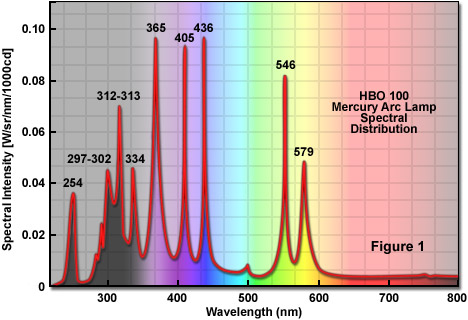
\includegraphics[width=10cm]{images/mercurylamp.jpg}
				\caption{Optical spectra of a mercury arc lamp, similar to the one used in the experiment.}
				\label{fig:mercuryspectra}
			\end{figure}
		
		\subsubsection{Optical Elements}
			\paragraph{Aperture}
				An aperture is a small opening that allows only a small portion of incident light to pass on through the other optical elements in the setup. 
				\begin{figure}[H]
					\centering
					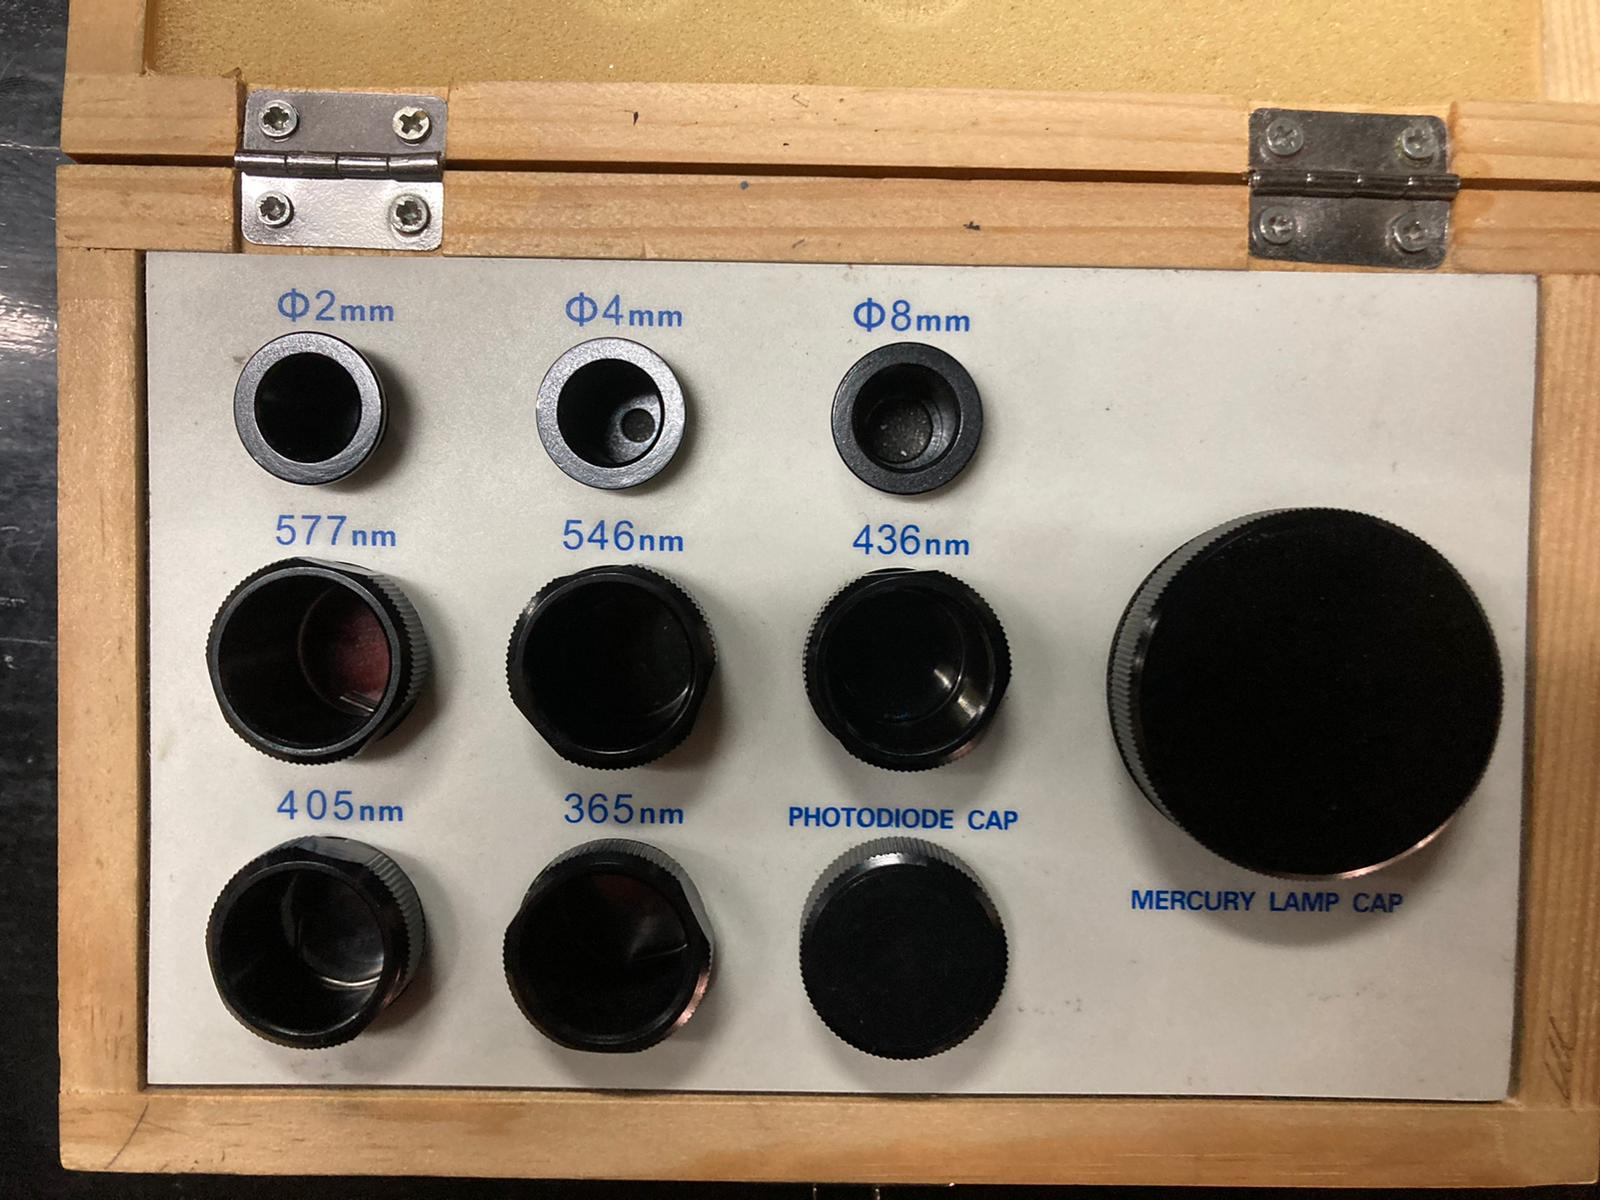
\includegraphics[width=10cm]{images/lens_aperture.jpeg}
					\caption{The optical elements used in this experiment. Apertures and optical filters.}
					\label{fig:opticalelements}
				\end{figure}
				An aperture with 4mm diameter was used throughout this experiment, which can be seen in Figure \ref{fig:opticalelements}
			\paragraph{Optical Filter}
				An optical filter is an optical device that only allows the selected wavelengths to pass on, while blocking all the other wavelengths.
				\\
				\\
				Five different optical filters were used throughout the experiment to produce output light with different wavelengths, them being: 365nm, 405nm, 436, nm, 546nm and 577nm. These wavelengths of the optical filters are directly correlated with the peaks in the optical spectra of the mercury arc lamp as it is shown in Figure \ref{fig:mercuryspectra}
		\subsubsection{Phototube}
			A phototube is a vacuum tube that is used to sense light that are mostly replaced by semiconductor photodetectors in recent years. The phototube contains a coated cathode and a circular anode inside which are crucial for the physics behind this experiment.
			\\
			\\
			The photocathode surface needs to be coated with a substance that has a low work function. The work function being uniform is an advantage as well, but a nonuniform work function can be mitigated by using apertures before the phototube, reducing the illuminated area on the photocathode.\\
			\\
			The anode is chosen to be in a ring shape to prevent any light from striking it directly. This still happens with a ring shaped anode but we can consider it as measurement error without worrying too much. 
			\begin{figure}[H]
				\centering
				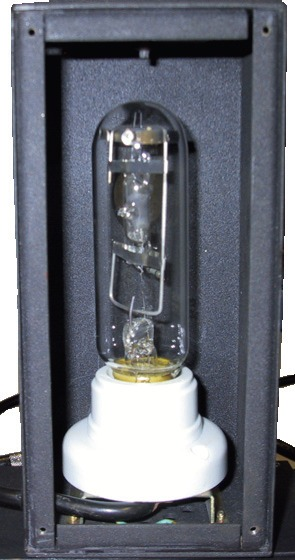
\includegraphics[width=5cm]{images/phototube.jpeg}
				\caption{The phototube used in the experiment, photo is taken with the casing off.}
				\label{fig:phototube}
			\end{figure}
			
	
	\subsection{Procedure}
	
		\subsubsection{Calibration Procedure}
			After turning on the mercury arc lamp and letting the setup warm up, we disconnected the anode, cathode and ground cables of the phototube and turned on the calibration mode of the photoelectric effect apparatus. While in the calibration mode, we aadjusted the current calibration node until the current was zero on the screen, turned the calibration mode off and connected the cables of the phototube.
		
		\subsubsection{Experiment Procedure}
			After the calibration, we placed the 4mm aperture and the necessary color filter in front of the phototube and first found the stopping voltage value where the current was zero, then adjusted the voltage knob to measure current values from the apparatus. We repeated this procedure for all of the color filters.
